\documentclass[12pt,english]{article}
%%% PREAMBLE

%%% Install missing packages %%%
% tinytex::parse_install("MainText.log")

% Sometimes you have to run: tinytex::install_tinytex()
% and maybe: tlmgr_update()

\usepackage{bbding} % for checkmark symbol
\usepackage{booktabs}
%\usepackage{chngcntr} % Allows table and figure counters to be reset in Appendix
\usepackage[font=small,format=hang,justification=raggedright,labelfont=up,labelsep=space,singlelinecheck=false]{caption}
\usepackage{color} % use to color text
\usepackage{enumitem}
  \setlist[enumerate]{itemsep=0mm}
\usepackage[T1]{fontenc}
\usepackage{geometry} % set margins and stuff
\usepackage{graphicx}
\usepackage{lineno}
\usepackage{longtable}
\usepackage{microtype}
\usepackage{pdflscape} % Causes pages that are in landscape format to be rotated when viewing the pdf but print as usual
\usepackage{scrextend} % Allows you to change margins for section of text
\usepackage{setspace}
\usepackage{siunitx}
\usepackage{titlesec}
\usepackage[dvipsnames]{xcolor} % use to get more colors

%\DisableLigatures{encoding = *, family = *}
\DisableLigatures[f]{encoding = *, family = *} %% <- only disables f-ligatures

\PassOptionsToPackage{hyphens}{url}\usepackage[hidelinks]{hyperref} % enables hyperlinks
\urlstyle{same} % Maintains URLs in the same font as the rest of the text

% Bibliography related
\usepackage{natbib}                            % For citations
\bibpunct{(}{)}{;}{a}{}{;}
\setlength{\bibhang}{2em}

%\addbibresource{KlibanskyFishResearch_1.5}
%\graphicspath{ {images/} }
\geometry{verbose,letterpaper,tmargin=2.54cm,bmargin=2.54cm,lmargin=2.54cm,rmargin=2.54cm}
%\linenumbers

\captionsetup{figurename=Fig.}

% Define heading formatting
\titleformat{\section}
   {\small\mdseries\scshape}{\thesection}{1em}{}

\titleformat{\subsection}
   {\small\mdseries\itshape}{\thesubsection}{1em}{}

%%% Main document
% BEGIN DOCUMENT
\usepackage{Sweave}
\begin{document}
\Sconcordance{concordance:MainText.tex:MainText.Rnw:%
1 56 1 1 0 2 1 1 9 1 11 1 5 1 14 273 1}







% Top matter
\title{Evaluating procedures for updating catch advice between stock assessments of reef fishes with management strategy evaluation}
\author{Nikolai Klibansky,  Shannon Calay, Rob Cheshire,\\
Cassidy Peterson, Kyle Shertzer, Erik Williams, and Matt Vincent\\\\
Southeast Fisheries Science Center, \\
National Marine Fisheries Service, NOAA,\\
101 Pivers Island Road, Beaufort, North Carolina, 28516, USA}
\maketitle

\begin{abstract}
We built operating models for three reef fish species from the US Southeast Atlantic, based on recent stock assessments. We developed 23 scenerios and 13 management procedures. Management procedures varied in terms of how often stock assessments were conducted, and how catch advice was adjusted between stock assessments.

\end{abstract}

\begin{flushleft}
\begin{spacing}{1.9}
\setlength{\parindent}{1cm} % Indent paragraphs after the first one

\section*{Introduction}
We can only do stock assessments every few years. It would be nice to know if there were ways that we could adjust catch advice between stock assessments to improve.


\section*{Materials and Methods}

\subsection*{Operating models}
We used the most recent stock assessments from US Southeast US Atlantic for Red Porgy, Black Sea Bass, Vermilion Snapper, and Snowy Grouper (cite SEDAR reports). Elements of the stock assessments are stored as data sets in the R package \texttt{bamExtras} (cite Github). Management strategy evaluation was conducted with the R package \texttt{openMSE} (cite), which includes three sub-packages \texttt{DLMtool}, \texttt{MSEtool}, and \texttt{SAMtool} (cite). This package uses a set of data objects with very specific list-like structures (S4; \url{http://adv-r.had.co.nz/S4.html}), such as operating model objects (\texttt{OM}). Such objects are made up of a set of named 'slots', which contain specific types of information with particular dimensions, to characterize main components of an MSE. Input and output from the Beaufort Assessment Model (BAM) is configured as a list which has a specific structure, and is stored in an \texttt{rdat} file. The most recent \texttt{rdat} files are also stored in \texttt{bamExtras} as objects (e.g. \texttt{rdat\_BlackSeaBass}). In order to the transfer information from BAM \texttt{rdat} objects to \texttt{openMSE} objects, we wrote a set of functions and constructed a new R package, \texttt{bamMSE} (cite GitHub).

Operating models in \texttt{openMSE} (\texttt{OM} class S4 objects) are constructed of four sub-objects: \texttt{Stock}, \texttt{Fleet}, \texttt{Obs}, and \texttt{Imp} class objects. Values stored in \texttt{Stock} objects describe a fish stock, \texttt{Fleet} objects characterize a fishing fleet that fishes that stock, \texttt{Obs} objects contain parameters describing how the simulated stock and fleet are observed (e.g. bias and error of catch or relative abundance data), and the \texttt{Imp} objects allow the user to set how well managers adhere to management recommendations (i.e. implementation error). A fifth \texttt{openMSE} object class \texttt{Data}, is used to store various types of data, including data sets typically used in fitting stock assessment models (e.g. indices of abundance, catch, and age-composition time series). Functions in \texttt{bamMSE} convert \texttt{rdat} objects to \texttt{Stock}, \texttt{Fleet}, \texttt{Obs}, and \texttt{Data} objects (\texttt{rdat2Stock}, \texttt{rdat2Fleet}, \texttt{rdat2Obs}, and \texttt{rdat2Data}).

We used the function \texttt{MSEtool::Assess2OM} to convert BAM results to \texttt{OM} objects, with the help of a wrapper function \texttt{bamAssess2OM} (not yet added to \texttt{bamMSE}). While the values of the steepness parameter $h$, and unfished recruitment ($R_{0}$) for the Beverton-Holt stock-recruit relationship is directly passed from BAM to \texttt{Assess2OM}, most other inputs had to be modified from BAM. Since \texttt{openMSE} requires the first age in age-structured populations to be age-0, and most BAM assessments start with age-1, age-based data from BAM was linearly extrapolated from age-1 to age-0 before being passed to \texttt{Assess2OM}. Such data include several three dimensional numeric arrays with dimensions simulation, age, and year (within recent assessment period): fish weight, fish length, proportion mature, numbers of fish, total fishing mortality rate ($F$; including dead discards) , and natural mortality rate ($M$).

We ran  \texttt{rdat2Data} on the \texttt{rdat} objects, and passed indices of abundance, their associated CVs, and selectivity-at-age to an \texttt{openMSE} \texttt{cpars} list object. In \texttt{openMSE} a \texttt{cpars} list object is used to pass custom parameters, typically time-varying, to an operating model. The \texttt{rdat2Data} function assumes that indices based on surveys or recreational fisheries are in numbers and indices based on commercial fisheries are in pounds. Only indices available in the terminal year of the assessments were passed to \texttt{cpars} and the \texttt{OM} objects (Fig. \ref{fig:AddInd}). Estimated of growth parameters ($K$, $L_{\infty}$, and $t_{0}$) from BAM were also passed to the \texttt{OM} objects. Selectivity-at-age of removals is estimated annually during the empirical assessment period by \texttt{Assess2OM}, and the average of the last three years of the assessment period was passed to \texttt{cpars} and the \texttt{OM} objects.

\subsection*{Scenarios}


\begin{enumerate}
\setstretch{1}
\item Base (base): Most likely scenario, described above

\item Episodic $M$ (epiM): $M$ is constant in most years but is occasionally much higher
\item Age-varying $M$ (agevarM): $M$ varies with age
\item Set $M$ (Mset): $M$ is set to the same fixed value for all species ($M$ = 0.2)
\item Set $h$ (steepset): $h$ is set to the same fixed value for all species ($h$ = 0.84)
\item Set life history (lhset): $M$ and $h$ are set to the same fixed values for all species ($M$ = 0.2, $h$ = 0.84)
\item Minimal rec. dev. (minrecdev): Recruitment deviations set to low value
\item Vulnerability time variant (vtvar): Selectivity associated with catch (i.e. vulnerability) varies annually during the historic period
\item Depleted (dep): Depletion of the stock is high (i.e. smaller stock size) at the beginning of the projection period
\item Lightly fished (lf): Depletion of the stock is low (i.e. larger stock size) at the beginning of the projection period.
\item Regime change (rc): Recruitment deviations decline over the projection period, then remain low

\item No empirical indices (noempind): No empirical indices, CVs, or index selectivities are included in the \texttt{OM}
\item Index is biased (ubias): Primary index of abundance increasingly underestimates population size (i.e. decreasing catchability)
\item Index high CV (ucvhi): Primary index of abundance of abundance is twice as high
\item Index low CV (ucvlo): Primary index of abundance of abundance is half as high
\item Hyper-deplete: Primary index of abundance is hyper-deplete
\item Hyper-stable: Primary index of abundance is hyper-stable
\item Minimal error (minerr): Minimal (but not zero) error in all stochastic elements of the \texttt{OM}
\item Perfect observation (perfobs): Minimal observation error and very high sample sizes in data sets

\item Vulnerability dome-shaped (vdome): Selectivity associated with catch (i.e. vulnerability) is estimated with a dome-shaped function in stock assessments
\item No data lag (nolag): Catch advice (i.e. TAC) from stock assessments is implemented the year after the terminal year of the assessment
\item High TAC (tachi): TAC = 1.25MSY
\item Low TAC (taclo): TAC = 0.75MSY
\end{enumerate}
\setstretch{2}

\subsection*{Management procedures}

\begin{enumerate}
\setstretch{1}
\item Average catch (AvC): Average catch over all years
\item Recent catch (CC1): Average catch over the last 5 years
\item Depletion corrected average catch (DCAC):
\item Depletion based stock reduction analysis (DBSRA):
\item Surplus production model (SPMSY):
\item Statistical catch-at-age model
\begin{enumerate}
\item 1-year interval (SCA\_1)
\item 5-year interval with fixed TAC between years (SCA\_5)
\item 10-year interval with fixed TAC between years (SCA\_10)
\item 5-year interval with projected TAC between years (pMP\_5)
\item 10-year interval with projected TAC between years (pMP\_10)
\item 5-year interval with TAC adjusted based on averaged recent index between years  (iMP\_avg\_5)
\item 10-year interval with TAC adjusted based on averaged recent index between years  (iMP\_avg\_10)
\item 5-year interval with TAC adjusted based on buffered averaged recent index between years  (iMP\_bfr\_5)
\item 10-year interval with TAC adjusted based on buffered averaged recent index between years  (iMP\_bfr\_10)
\end{enumerate}
\end{enumerate}
\setstretch{2}

\subsection*{Response variables and performance metrics}

(include description of stock assessments and interim approach calculations)

Response variables: Catch, average annual variability in catch, $SSB/SSB_{MSY}$, $F/F_{MSY}$.

\section*{Results}

Response variables tended to vary among time periods over the projection years, and therefore plotted by time period.
In general, stock status ($SSB/SSB_{MSY}$) was similar among all nine SCA-based MPs for all four species, pooling across scenarios (Fig. \ref{fig:boxplotSBSBMSY1}). However MPs that adjusted between assessments with a buffered index approach tended to show slightly higher stock status for Black Sea Bass and Vermilion Snapper. Fishery status ($F/F_{MSY}$) was somewhat more variable, but still largely consistent among SCA-based MPs, for all species. For Black Sea Bass and Vermilion Snapper, $F/F_{MSY}$ for buffered index MPs tended to be at the low end of the range of the other MPs. Similarly, total catch was also similar among SCA-based MPs for all species, for similar time periods. Average annual variability in yield (catch) showed more substantial variation among MPs.


\section*{Discussion}

Some broad conclusions

Which factors seem to account for the most variation in results in general?
\begin{itemize}
\item Above all, results differ between operating models (i.e. species)
\item Scenario is the next most important factor, particularly depletion scenarios and regime change
\end{itemize}

\section*{Acknowledgements}
We thank everyone.

\end{spacing}
\end{flushleft}

% \printbibliography
%%% LITERATURE CITED %%%
%\printbibliography
\clearpage
\section*{Literature Cited}
\renewcommand{\refname}{}
\bibliographystyle{ecosphere} % Modified from ecology.bst
\vspace{-1cm}

\bibliography{KlibanskyFishResearch_1.5}


%% TABLES
\newpage
\section*{Tables}

%\input{../Results/biodivByArea.tex}
%\clearpage


%% FIGURES %%
\newpage
\section*{Figures}

% Indices
\begin{figure}[!ht]
\begin{center}
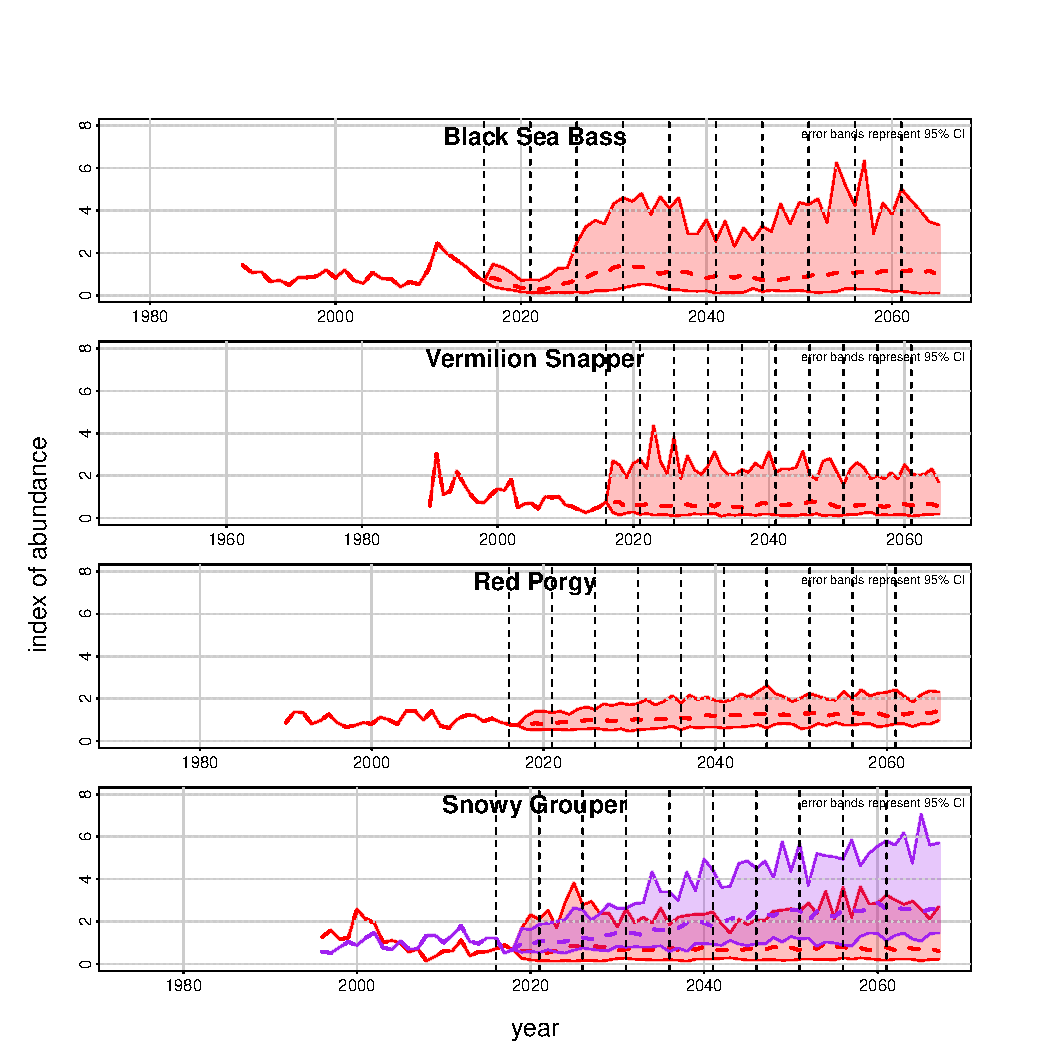
\includegraphics[width=6in,height=7in]{../Figs/AddInd.pdf}
\end{center}
\begin{flushleft}
\caption{Indices derived from BAM stock assessments available during the projection period, for the SCA\_10 MP in the Base scenario, where stock assessments are conducted every 10 years during the projection period (dashed vertical lines). Shaded areas represent 95\% CI for indices among simulation runs.}
\label{fig:AddInd}
\end{flushleft}
\end{figure}

% Boxplot of SSB/SSBMSY 1
\begin{figure}[!ht]
\begin{center}
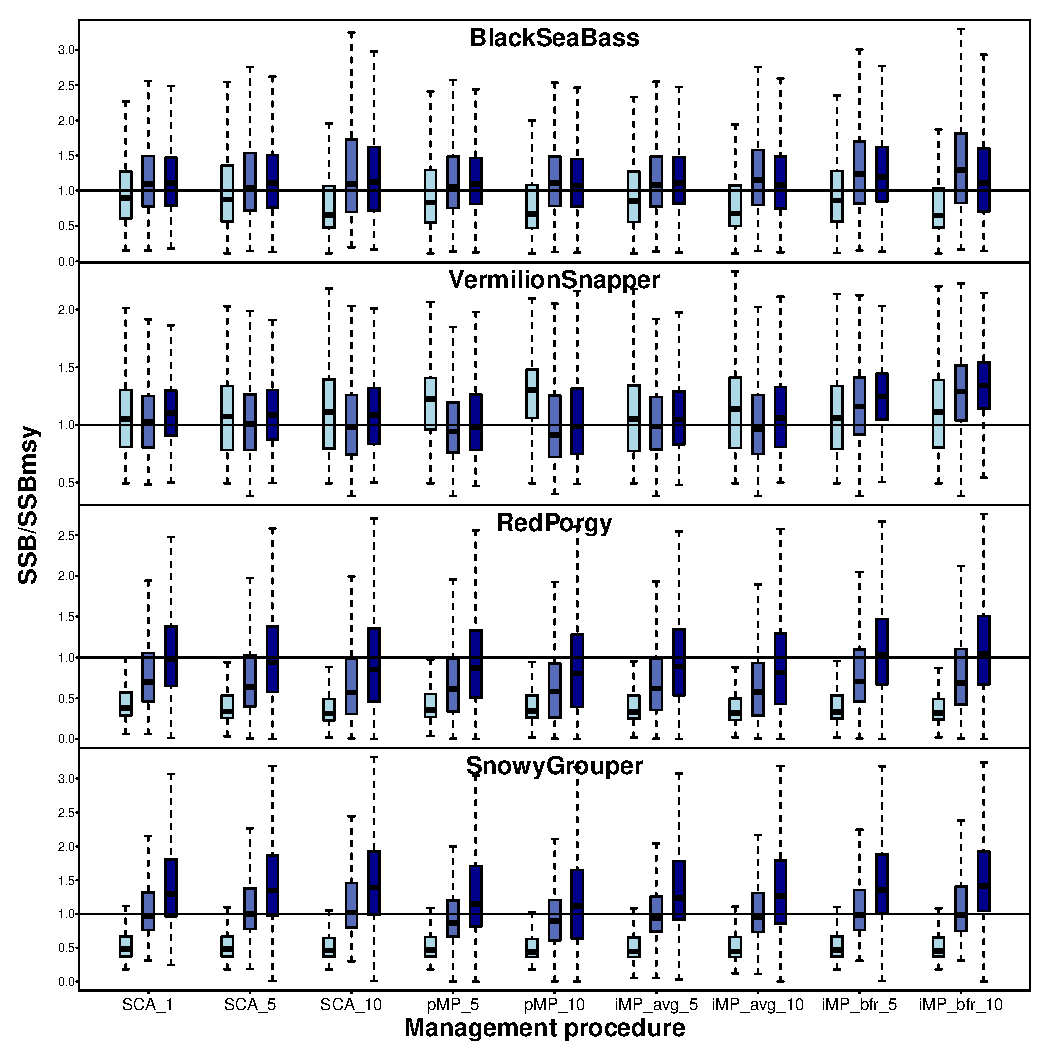
\includegraphics[width=6in,height=7in]{../Figs/boxplotSBSBMSY1.pdf}
\end{center}
\begin{flushleft}
\caption{Box plots of $\mathrm{SSB/SSB_{MSY}}$ for the base and alternative scenarios. Grouped boxes represent sequential time periods during the projection period.}
\label{fig:boxplotSBSBMSY1}
\end{flushleft}
\end{figure}

% Boxplot of F/FMSY 1
\begin{figure}[!ht]
\begin{center}
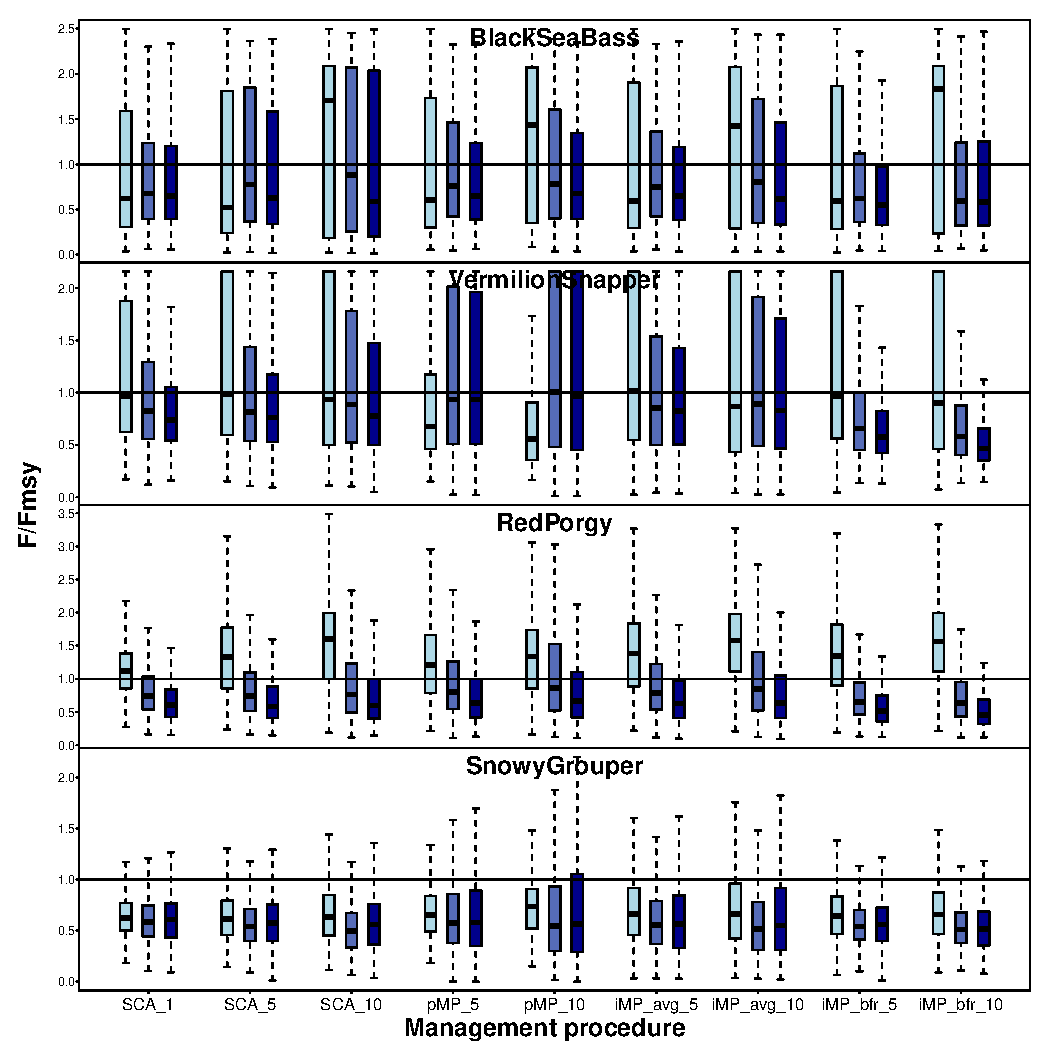
\includegraphics[width=6in,height=7in]{../Figs/boxplotFFMSY1.pdf}
\end{center}
\begin{flushleft}
\caption{Box plots of $\mathrm{F/F_{MSY}}$ for the base and alternative scenarios. Grouped boxes represent sequential time periods during the projection period.}
\label{fig:boxplotFFMSY1}
\end{flushleft}
\end{figure}

% Boxplot of Catch 1
\begin{figure}[!ht]
\begin{center}
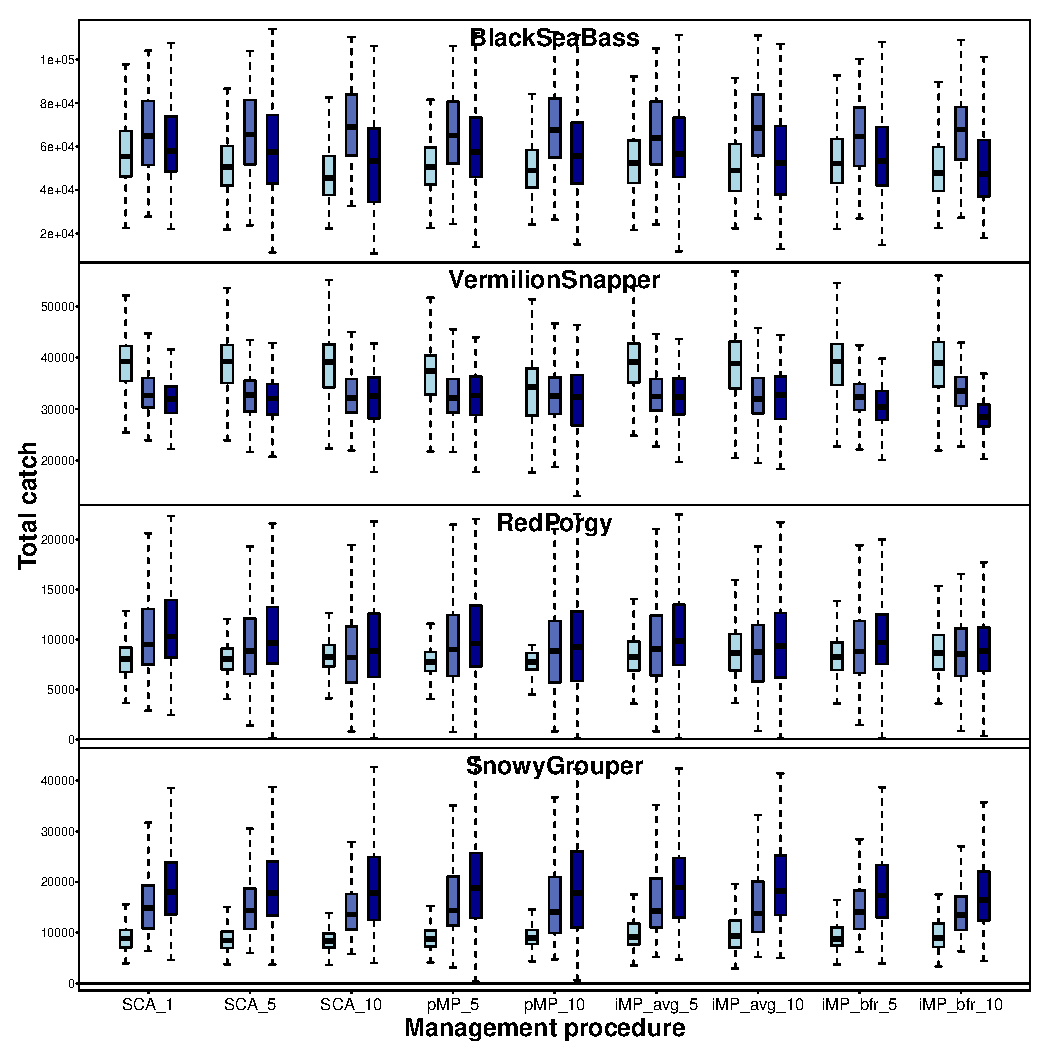
\includegraphics[width=6in,height=7in]{../Figs/boxplotCatchTotal1.pdf}
\end{center}
\begin{flushleft}
\caption{Box plots of total catch (annual catches summed across each time period), for the base and alternative scenarios. Grouped boxes represent sequential time periods during the projection period.}
\label{fig:boxplotCatch1}
\end{flushleft}
\end{figure}

% Boxplot of AAVY 1
\begin{figure}[!ht]
\begin{center}
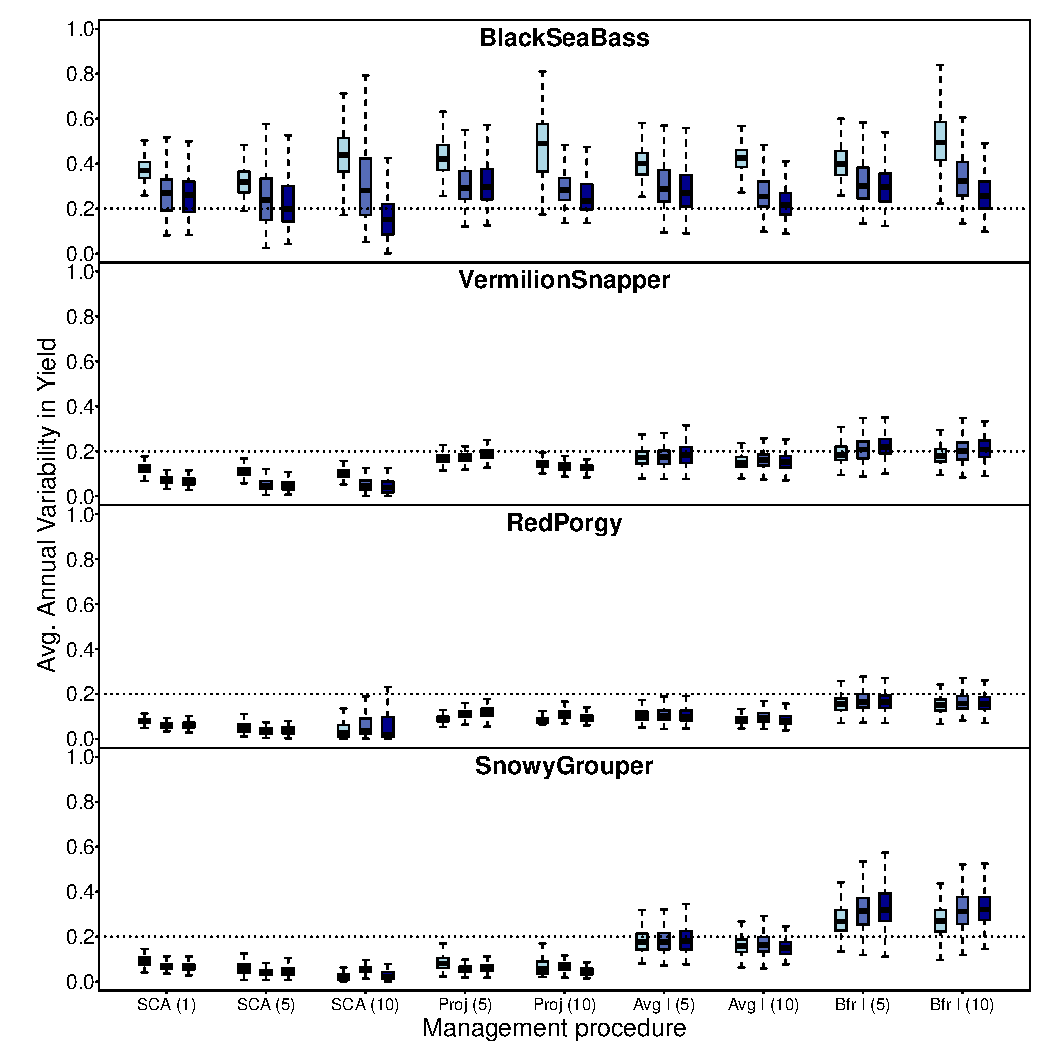
\includegraphics[width=6in,height=7in]{../Figs/boxplotAAVY1.pdf}
\end{center}
\begin{flushleft}
\caption{Box plots of average annual variation in yield ($\mathrm{AAVY}$) for the base and alternative scenarios. Grouped boxes represent sequential time periods during the projection period.}
\label{fig:boxplotAAVY1}
\end{flushleft}
\end{figure}

% Time series of SSB/SSBMSY 1
\begin{figure}[!ht]
\begin{center}
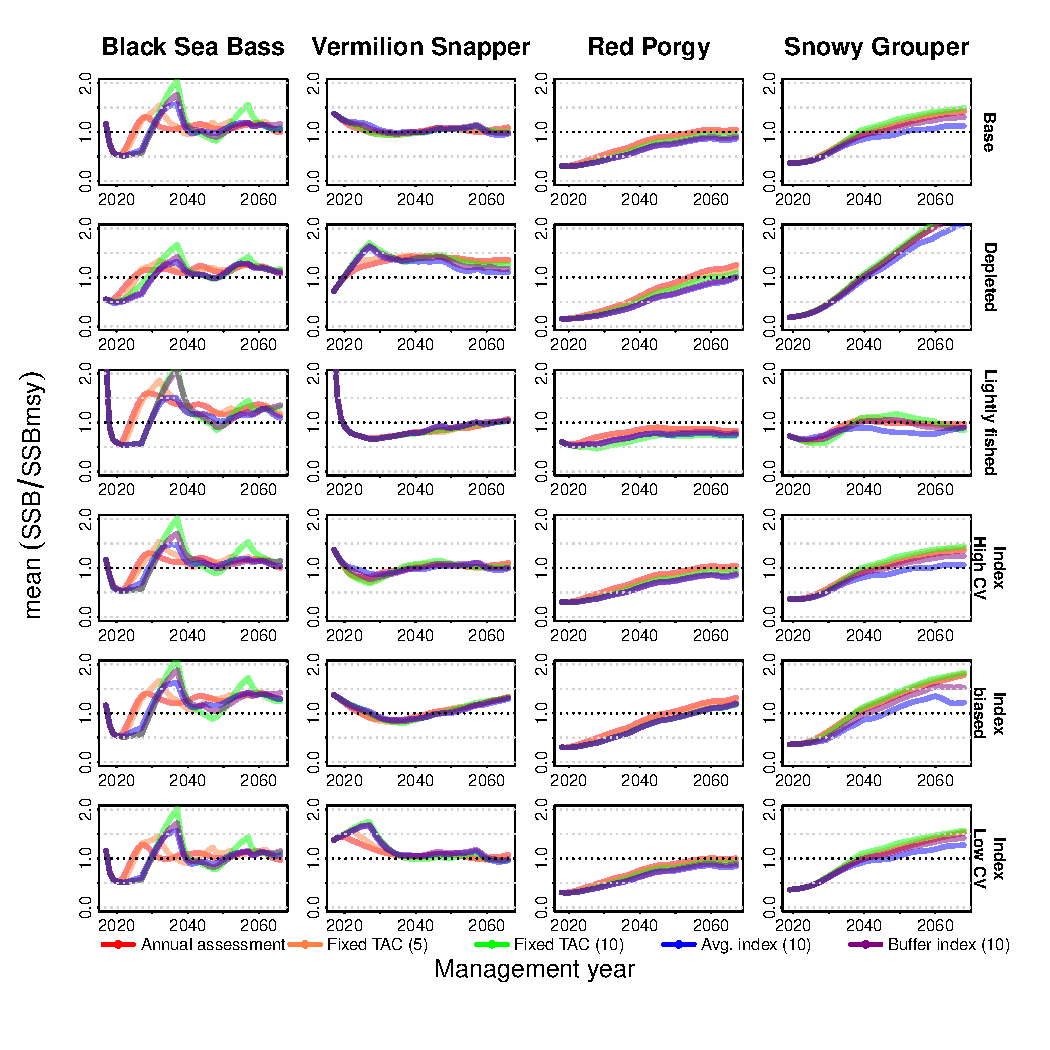
\includegraphics[width=6in,height=7in]{../Figs/tsSSBSSBmsy1.pdf}
\end{center}
\begin{flushleft}
\caption{Time series of mean $\mathrm{SSB/SSB_{MSY}}$ among simulation runs for the base and alternative scenarios. }
\label{fig:tsSSBSSBmsy1}
\end{flushleft}
\end{figure}

% Time series of F/FMSY 1
\begin{figure}[!ht]
\begin{center}
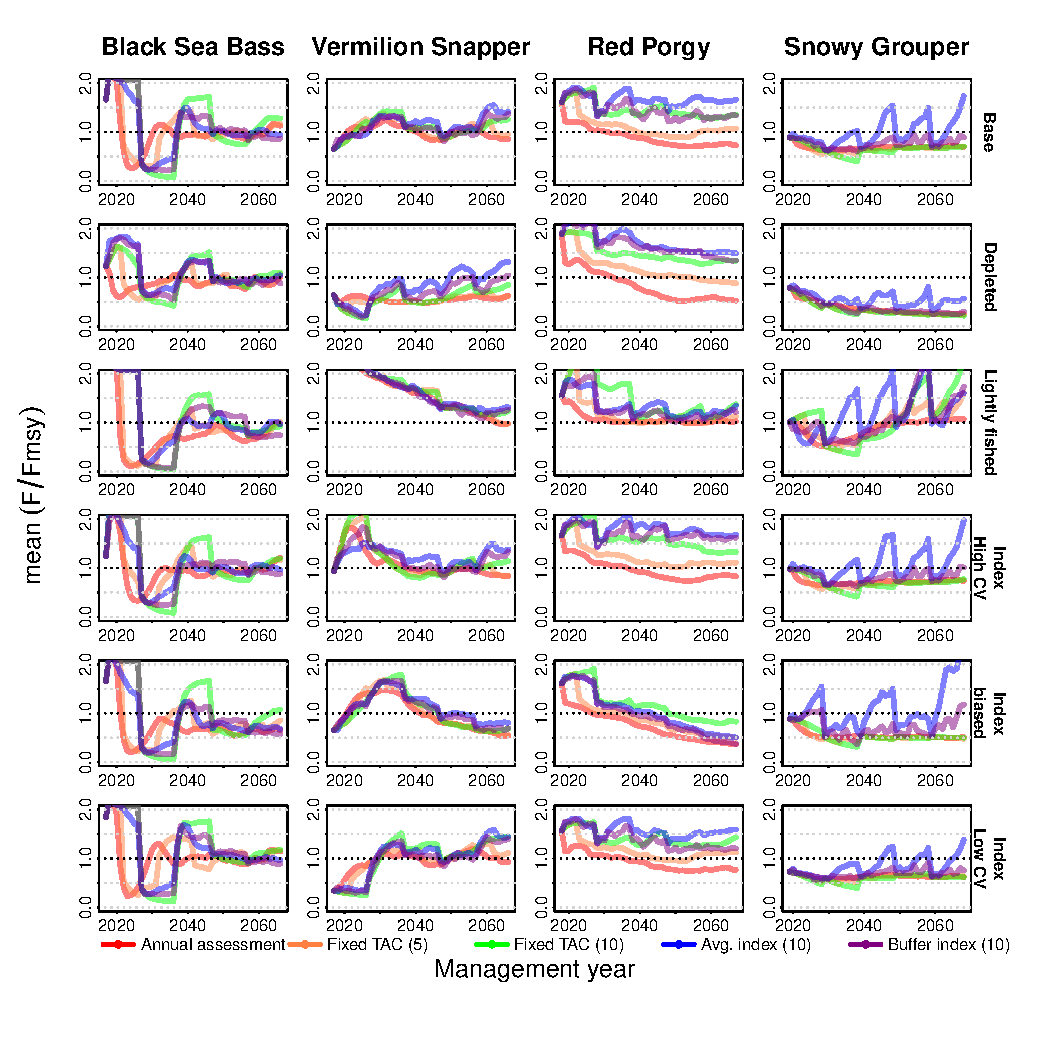
\includegraphics[width=6in,height=7in]{../Figs/tsFFmsy1.pdf}
\end{center}
\begin{flushleft}
\caption{Time series of mean $\mathrm{F/F_{MSY}}$ among simulation runs for the base and alternative scenarios. }
\label{fig:tsFFmsy1}
\end{flushleft}
\end{figure}

% Time series of Catch 1
\begin{figure}[!ht]
\begin{center}
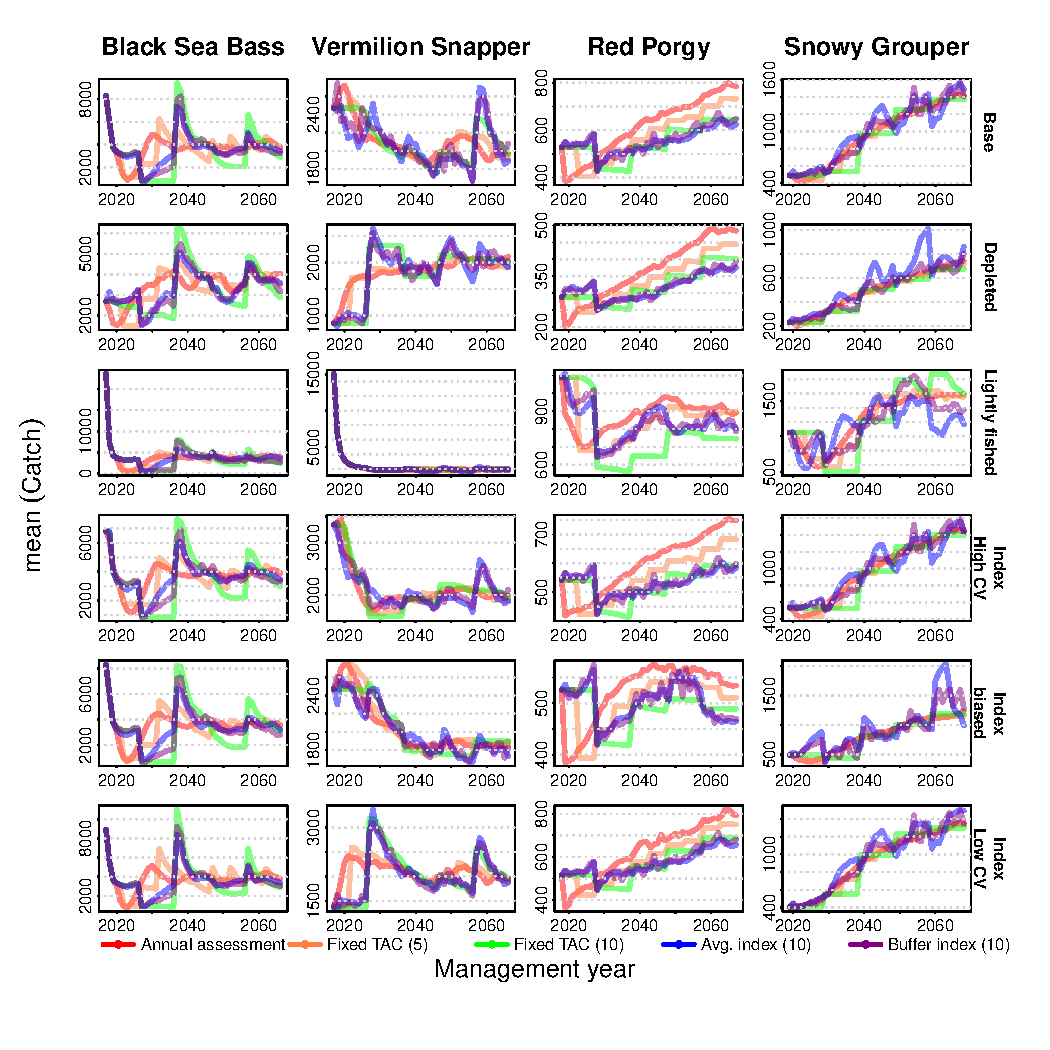
\includegraphics[width=6in,height=7in]{../Figs/tsCatch1.pdf}
\end{center}
\begin{flushleft}
\caption{Time series of mean $\mathrm{catch}$ among simulation runs for the base and alternative scenarios. }
\label{fig:tsCatch1}
\end{flushleft}
\end{figure}


% Phase plots
\begin{figure}[!ht]
\begin{center}
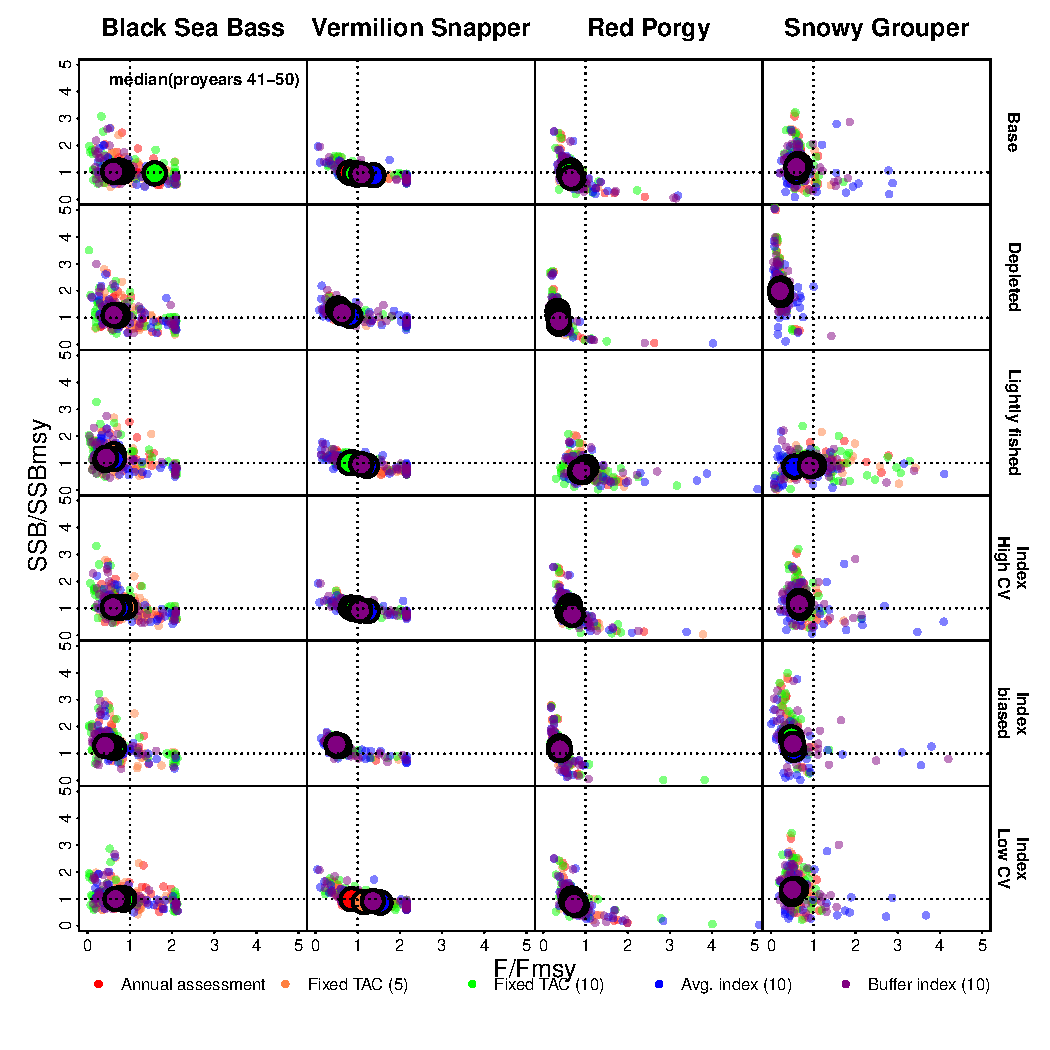
\includegraphics[width=6in,height=7in]{../Figs/phasePlot1.pdf}
\end{center}
\begin{flushleft}
\caption{Phase plots for the base and alternative scenarios.}
\label{fig:phasePlot1}
\end{flushleft}
\end{figure}

% \begin{figure}[!ht]
% \begin{center}
% 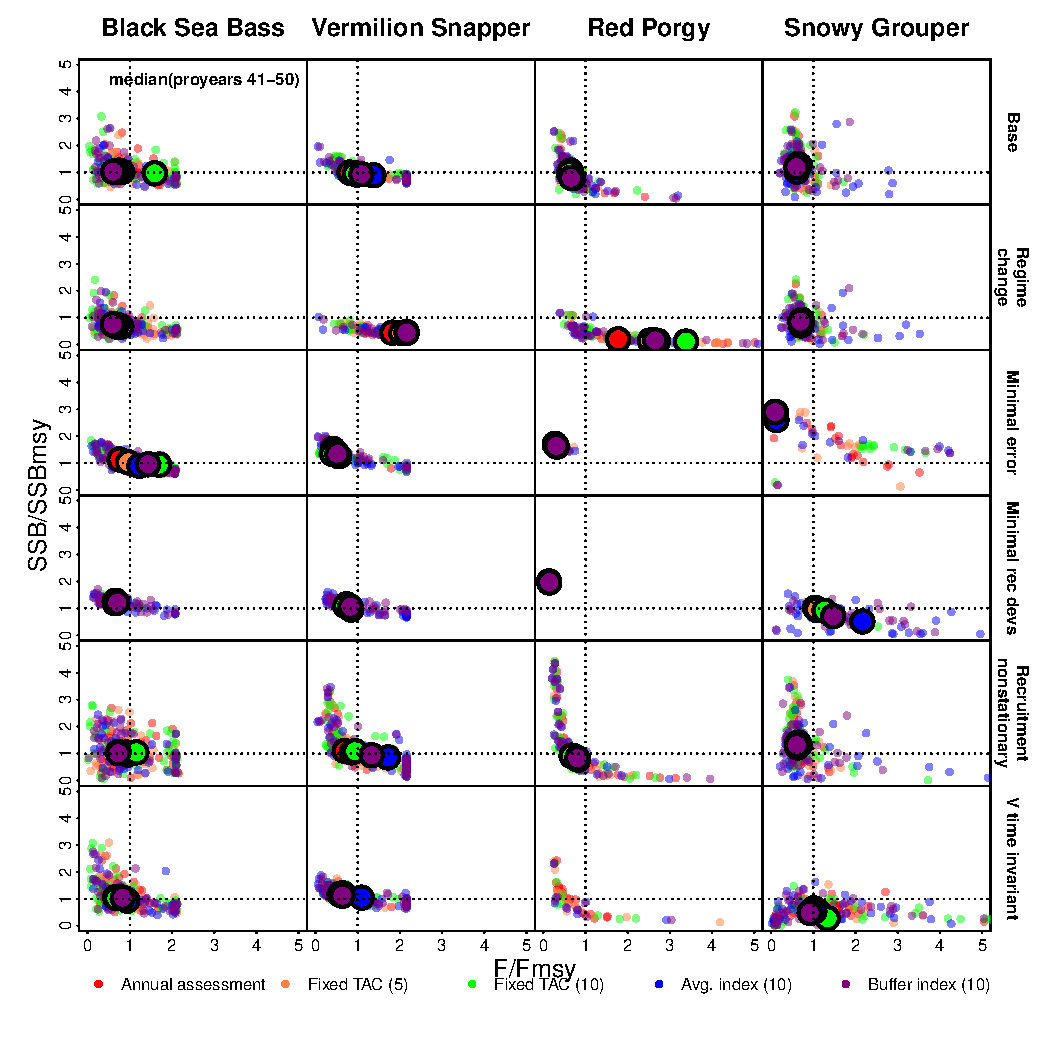
\includegraphics[width=6in,height=7in]{../Figs/phasePlot2.pdf}
% \end{center}
% \begin{flushleft}
% \caption{Phase plots for the base scenario and the second set of experimental scenarios}
% \label{fig:phasePlot2}
% \end{flushleft}
% \end{figure}


%% APPENDIX
% \begin{appendix}
%
% \clearpage
% \section*{Appendix S1}
%
% \setcounter{table}{0}
% \renewcommand{\thetable}{S\arabic{table}}
%
% \input{../Results/Appendix.tex}
%
% \input{../Results/biodivByBlock.tex}
%
% \end{appendix}


% END DOCUMENT
\end{document}
